\documentclass[a4paper,landscape,twocolumn]{article}
\usepackage[utf8]{inputenc}
\usepackage[T1]{fontenc}
\usepackage[ngerman,english]{babel}
\usepackage{amsmath}
\usepackage{amssymb}
\usepackage{amsthm}
\usepackage{csquotes}
\usepackage{fancyhdr}
\usepackage[margin=1in]{geometry}
\usepackage[makeindex]{imakeidx}  % before hyperref
\usepackage[pdfborder={0 0 0}]{hyperref}
\usepackage{marvosym}
\usepackage{mathtools}
\usepackage{mdframed}
\usepackage{stmaryrd}
\usepackage[normalem]{ulem}
\usepackage{wasysym}

\parskip5pt
\parindent0pt

\theoremstyle{definition}

\newtheorem{theorem}{Theorem}
\newtheorem{defi}{Definition}
\newtheorem{rem}{Remark}
\newtheorem{ex}{Example}
\newtheorem{cor}{Corollary}
\newtheorem{lemma}{Lemma}

\newcommand\okay{\qquad\checkmark}
\newcommand\set[1]{\left\{#1\right\}}
\newcommand\setdef[2]{\left\{#1\,|\,#2\right\}}
\newcommand\abs[1]{\left|#1\right|}
\newcommand\seq[1]{{\left(#1\right)}_{n \in \mathbb N}}
\newcommand\card[1]{\left|\,#1\,\right|}
\newcommand\meta[3]{\hrule{} This #1 took place on #2 with lecturer #3.\par}
\newcommand\done{\hspace{10pt}\checkmark}
\newcommand\norm[1]{\left\|#1\right\|}

\pagestyle{fancy}
\fancyhf{}
\chead{\Large{\textsc{Mathematical Analysis II -- Lecture Notes}}}
\lfoot{\makebox[\columnwidth]{\thepage}}
\rfoot{\makebox[\columnwidth]{\number\numexpr\value{page}+1}\stepcounter{page}}
\setlength{\headheight}{18pt}

\makeindex[name={German},title={German keywords}]
\makeindex[name={English},title={English keywords}]
\twocolumn

\title{
  Mathematical analysis 2 -- Lecture notes \\
  \small{course by Wolfgang Ring}
}
\author{Lukas Prokop}
\date{March to July 2016}

\begin{document}
\maketitle
\tableofcontents

\clearpage
\meta{lecture}{1st of March 2016}{Wolfgang Ring}

Course organization:
\begin{itemize}
  \item Tuesday, 1 hours 30 minutes, beginning at 8:15
  \item Thursday, 45 minutes, beginning at 8:15
  \item Friday, 1 hours 30 minutes, beginning at 8:15
\end{itemize}

Literature:
\begin{itemize}
  \item Königsberger, Analysis 1
\end{itemize}

\clearpage
\section{Exponential function (cont.)}
%
Let $(z_n)_{n \in \mathbb N}$ be a complex series with $\lim_{n\to\infty} z_n = z$
and $\lim_{n\to\infty} (1 + \frac{z_n}{n})^n = \sum_{k=0}^\infty \frac{z^k}{k!}$.
For every complex number $z \in \mathbb C$ this series converges on entire $\mathbb C$.

\[ \exp(z) = \lim_{n\to\infty} \left(1 + \frac{z}n\right)^n = \sum_{k=0}^\infty \frac{z^k}{k!} \]
\[ \exp(z + w) = \exp(z) \cdot \exp(w) \]
\[ \lim_{z\to0} \frac{\exp(z) - 1}{z} = 1 \]
\[ \exp(1) = e \in \mathbb R \]
\[ z = \frac mn \in \mathbb Q \land n \neq 0 \Rightarrow \exp\left(\frac mn\right) = e^{\frac mn} \]

So we also denote
\[ \exp(z) = e^z \qquad \text{for } z \in \mathbb C \]
It holds that
\[ \exp(z) \neq 0 \qquad \forall z \in \mathbb C \]

$\exp(x)$ for $x \in \mathbb R$
\[ e^x > 0 \qquad \forall x \in \mathbb R \]

\[ (e^x)' = e^x \]
It follows immediately that the exponential function is strictly monotonically increasing in $\mathbb R$.
\[ (e^x)'' = (e^x)' = e^x > 0 \]
It follows that the exponential function is convex. But as usual,
\[ e^0 = 1 \]

\begin{figure}[!h]
  \begin{center}
    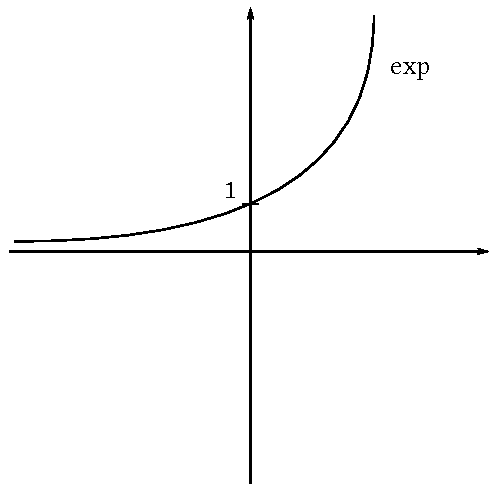
\includegraphics{img/exp-graph.pdf}
    \caption{Graph of the exponential function}
  \end{center}
\end{figure}

Let $n \in \mathbb N$
\[ \lim_{x\to+\infty} \frac{e^x}{x^n} = \infty \]
\[ \lim_{x\to-\infty} e^x \cdot x^n = 0 \]

\section{The natural logarithm}
%
\[ \exp: \mathbb R \to (0,\infty) \]
is injective, because $x_1 < x_2 \Rightarrow e^{x_1} < e^{x_2}$

\begin{lemma}
  $\exp: \mathbb R \to (0,\infty)$
  is surjective.
\end{lemma}
\begin{proof}
  We need to show that the equation $e^x = y$ has some solution for every $y > 0$.
  We will use the Intermediate Value Theorem, we discussed in the previous course \enquote{Analysis 1}.

  \begin{description}
    \item[Case 1]
      First of all, let $y \in [1,\infty)$. Then it holds that
      \[ e^0 = 1 \leq y \quad\text{and}\quad e^y = 1 + y + \underbrace{\frac{y^2}{2} + \frac{y^3}{3!} + \frac{y^4}{4!} + \ldots}_{\geq 0} \]
      \[ \geq 1 + y > y \]
      Therefore $e^0 \leq y < e^y$.
      Hence $\exp$ is continuous and the Intermediate Value Theorem applies:
      \[ \exists \xi \in [0,y]: \quad e^\xi = y \]
    \item[Case 2]
      Let $y \in (0,1)$. Then it holds that $w = \frac1{y} > 1$.
      The same as in Case~1 applies:
      \[ \exists \xi \in [0,w]: \quad e^\xi = w = \frac1{y} \]
      \[ \Rightarrow e^{-\xi} = \frac{1}{e^\xi} = y \]
  \end{description}

  So it holds that $\exp: \mathbb R \to (0,\infty)$ is bijective.
\end{proof}

\index[English]{Natural logarithm}
\index[German]{\foreignlanguage{ngerman}{Natürlicher Logarithmus}}
\begin{defi}
  We call the inverse function \emph{natural logarithm}\footnote{In non-German literature $\ln(y)$ is almost exclusively written with the more general $\log(y)$.}.
  \[ \exp^{-1}: (0,\infty) \to \mathbb R \]
  \[ \exp^{-1} = \ln(y) = \log(y) \]

  Properties:
  \begin{itemize}
    \item It holds $\forall x \in \mathbb R: \ln(e^x) = x$ and $\forall y \in (0,\infty): e^{\ln(y)} = y$.
    \item $\ln: (0,\infty) \to \mathbb R$ is strictly monotonically increasing
      \begin{proof}
        Let $0 < y_1 < y_2$. Assume $\ln(y_1) \geq \ln(y_2) \xRightarrow{\text{monotonicity}} e^{\ln(y_1)} \geq e^{\ln(y_2)} \Rightarrow y_1 \geq y_2$. Contradiction!
      \end{proof}
  \end{itemize}
\end{defi}

\subsection{Functional equations of logarithm}
%
\begin{itemize}
  \item
    For all $x,y > 0$ it holds that
    \[ \ln(x \cdot y) = \ln(x) + \ln(y) \]
  \item Limes:
    \[ \lim_{x \to 1} \frac{\ln(x)}{x - 1} = 1 \]
\end{itemize}
\begin{proof}
  \begin{itemize}
    \item
      \[ x \cdot y = e^{\ln(x \cdot y)} \]
      \[ e^{\ln(x)} \cdot e^{\ln(y)} = e^{\ln(x) + \ln(y)} \]
      Injectivity of $\exp$:
      \[ \ln(x \cdot y) = \ln(x) + \ln(y) \]
    \item
      Let $(x_n)_{n\in\mathbb N}$ with $x_n > 0$ be an arbitrary
      sequence with $\lim_{n\to\infty} x_n = 0$.
      Let $w_n = 1 + x_n$. Then it holds that
      $\lim_{n\to\infty} w_n = 1$ and $y_n = \ln(1 + x_n) = \ln(w_n)$.
      \[ \lim_{n\to\infty} y_n = \ln(1) = 0 \]
      \[ \lim_{n\to\infty} \frac{\ln(w_n)}{w_n - 1} = \lim_{n\to\infty} \frac{y_n}{e^{y_n} - 1} = \frac11 = 1 \]
      where
      \[ e^0 = 1 \Rightarrow \ln(1) = 0 \]
  \end{itemize}
\end{proof}

\begin{theorem}[Logarithmic growth]
  $\forall n \in \mathbb N_+$ it holds that $\lim_{n\to\infty} \frac{\ln(x)}{\sqrt[n]{x}} = 0$
\end{theorem}
\begin{proof}
  Let $x \in (0,\infty)$ with $x = e^{n\cdot\xi}$. That is,
  \[ \xi = \frac{\ln(x)}{n} \]
  \[ x \to \infty \Leftrightarrow \xi \to \infty \]
  \[
    \lim_{x\to\infty} \frac{\ln(x)}{\sqrt[n]{x}}
    = \lim_{\xi\to\infty} \frac{n \cdot \xi}{\sqrt[n]{e^{n \cdot \xi}}}
    = \lim_{\xi\to\infty} \frac{n \cdot \xi}{e^\xi} = 0
  \]
  because $n \cdot \xi < \xi^2$ for $\xi > n$ and $\lim_{\xi\to\infty} \frac{\xi^2}{e^\xi} = 0$.
\end{proof}

\begin{theorem}
  The logarithm function is differentiable in $(0,\infty)$ and it holds that $(\ln(x))' = \frac1x \quad \forall x > 0$.
\end{theorem}
\begin{figure}[!h]
  \begin{center}
    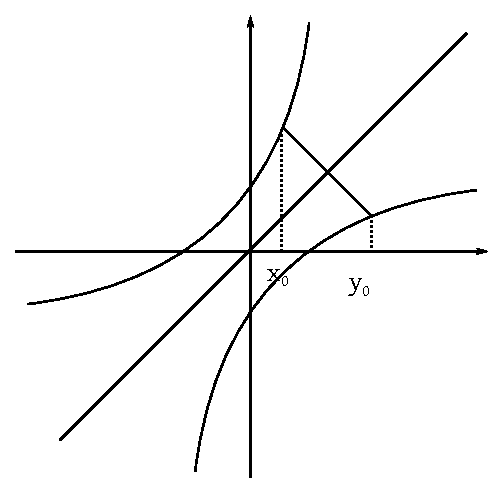
\includegraphics{img/geometric-exp-proof.pdf}
    \caption{A geometric proof of differentiability}
    \label{img:geo-diff}
  \end{center}
\end{figure}
\begin{proof}
  \begin{description}
    \item[First approach]
      Let $x > 0$, $x_n \to x$ with $x_n \neq x$, $x_n > 0$.
      Let $\xi_n = \ln(x_n)$ and $\xi = \ln(x) \Rightarrow \xi_n \neq \xi$.
      \[ e^{\xi_n} = x_n \qquad e^\xi = x \qquad \xi_n \to \xi \]
      Then it holds that
      \[ \lim_{n\to\infty} \frac{\ln(x_n) - \ln(x)}{x_n - x} = \lim_{n\to\infty} \frac{\xi_n - \xi}{e^{\xi_n} - e^\xi} \]
      \[
        = \lim_{n\to\infty} \frac{1}{\frac{e^{\xi_n} - e^\xi}{\xi_n - \xi}}
        = \frac{1}{\underbrace{\lim_{n\to\infty} \frac{e^{\xi_n} - e^\xi}{\xi_n - \xi}}_{(e^\xi)' = e^\xi}}
        = \frac1{e^\xi} = \frac1x
      \]
    \item[Second approach using chain rule]
      Compare with Figure~\ref{img:geo-diff}.
      \[ (f^{-1})'(y_0) = \frac{1}{f'(f^{-1}(y_0))} \]
      \[ f(f^{-1}(y)) = y \Rightarrow f(f^{-1}) f(f^{-1}(y)) = y = f'(f^{-1}(y)) \cdot (f^{-1})'(y) = 1 \]
      \[ \Rightarrow (f^{-1})'(y) = \frac{1}{f'(f^{-1}(y))} \text{ for } f(x) = \exp(x) \]
      \[ \Rightarrow (\ln)'(y) = \frac{1}{\exp(\ln(y))} = \frac{1}{y} \]

      \[ f(f^{-1}(y)) = y \]
      \[ f'(f^{-1}(y)) \cdot (f^{-1}) \]
      \[ = (f^{-1})'(y) = \frac{1}{f'(f^{-1}(y))} \]
      again for $f(x) = \exp(x)$.
    \item[Third approach]
      Let $x > 0$.
      \[ 0 = \ln(1) = \ln\left(x \cdot \frac1x\right) = \ln(x) + \ln\left(\frac1x\right) \]
      \[ \Rightarrow \ln\left(\frac1x\right) = -\ln(x) \]

      Let $x,y > 0$. Then it holds that
      \[ \ln{\frac{x}{y}} = \ln(x) - \ln(y) \]
      because $\ln\frac{x}{y} = \ln(x \cdot \frac1y) = \ln(x) - \ln(y)$.
  \end{description}
\end{proof}

\subsection{Extension of the functional equation of logarithm}
%


\subsection{A different proof for the derivative of logarithm}
%
\begin{proof}
  \[
    [\ln(x)]'
    = \lim_{h\to0} \frac{\ln(x + h) - \ln(x)}{h}
    = \lim_{h\to0} \frac{\ln\left(\frac{x+h}{x}\right)}{h}
    = \lim_{h\to0} \frac{\ln\left(1 + \frac{h}{x}\right)}{x \cdot \frac hx}
  \] \[
    = \frac1x \cdot \lim_{h\to0} \frac{\ln\left(1 + \frac{h}{x}\right)}{\frac{h}{x}}
    \text{ where } \frac hx \to 0
  \]
  $1 + \frac{h}{x} = w$ then it holds that $h \to 0 \Rightarrow w \to 1$.
  \[ \frac{h}{x} = w - 1 \]
  \[ \lim_{h\to0} \frac{\ln\left(1 + \frac{h}{x}\right)} = \lim_{h\to0} \frac{\ln(w)}{w - 1} = 1 \]
\end{proof}

\begin{rem}
  The exponential function can be defined from $\mathbb C$ to $\mathbb C$.
  \[ \exp: \mathbb C \to \mathbb C \]
  It is not possible to define the logarithm \emph{continuously} in entire $\mathbb C$
  (or $\mathbb C \setminus \set{0}$). We can only define a continuous inverse function
  of $\exp$ in $\mathbb C \setminus \set{x \in \mathbb R: x \leq 0}$
\end{rem}

\begin{figure}[!h]
  \begin{center}
    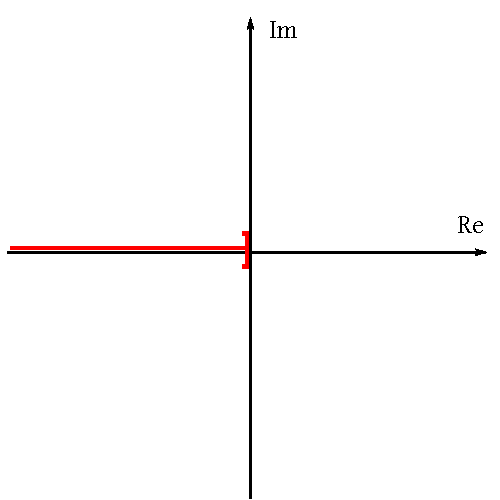
\includegraphics{img/continuous-exp-in-C.pdf}
    \caption{Continuous exponential function in $\mathbb C$}
  \end{center}
\end{figure}

\meta{lecture}{3rd of March 2016}{Wolfgang Ring}

\subsection{Further remarks on differential calculus}

\begin{theorem}
  Let $f: I \to \mathbb R$ be strictly monotonically increasing (or s. m. decreasing)
  where $I$ is an interval. Then $f^{-1}: f(I) \to \mathbb R$ is defined and the inverse function.

  Let $f$ in $x_0 \in I$ be differentiable and $f'(x_0) \neq 0$. Then $f^{-1}$ is in $y_0 = f(x_0)$
  differentiable and it holds that
  \[ (f^{-1})'(y_0) = \frac{1}{f'(x_0)} = \frac{1}{f'(f^{-1}(y_0))} \]
\end{theorem}

\begin{proof}
  Let $y_n \to y_0$ and $y_n \in f(I)$; $y_0 = f(x_0)$; $y_0 \in f(I)$; $y_n = f(x_n)$.
  $y_n \neq y_0 \Rightarrow x_n \neq x_0$.
  \[ \lim_{n\to\infty} \frac{f^{-1}(y_n) - f^{-1}(y_0)}{y_n - y_0} \]
  \[
    = \lim_{n\to\infty} \frac{x_n - x_0}{f(x_n) - f(x_0)}
    = \frac{1}{\lim_{n\to\infty} \underbrace{\frac{f(x_n) - f(x_0)}{x_n - x_0}}}_{\text{ex} = f'(x_0)} = \frac{1}{f'(x_0)}
  \]
\end{proof}

\begin{lemma}
  \label{lemma:const-diff}
  Let $f: I \to \mathbb R$ where $I$ is some interval. Then it holds that
  \[ f = \text{ const} \Leftrightarrow f \text{ is differentiable in $I$ and } f'(x) = 0 \forall x \in I \]
\end{lemma}
\begin{proof}
  \begin{description}
    \item[$\Rightarrow$]
      Immediate.
    \item[$\Leftarrow$]
      Let $f$ be differentiable and $f' \equiv 0$.
      Assume $f$ is not constant. Then there exist $x_1, x_2 \in I$, $x_1 \neq x_2$
      and $f(x_1) \neq f(x_2)$. Without loss of generality, $x_1 < x_2$.
      The Intermediate Value Theorem states that
      \[ \exists \xi \in (x_1, x_2) \subseteq I: f'(\xi) = \frac{f(x_2) - f(x_1)}{x_2 - x_1} \neq 0 \]
      This is a contradiction to the assumption that $f' \equiv 0$.
  \end{description}
\end{proof}

\index[English]{Primitive}
\index[German]{\foreignlanguage{ngerman}{Stammfunktion}}
\begin{defi}
  Let $I$ be an interval, $f: I \to \mathbb R$.
  A function $F: I \to \mathbb R$ is called \emph{primitive} or \emph{antiderivative} of $f$
  if $F$ is differentiable and
  \[ \forall x \in I: F'(x) = f(x) \]
\end{defi}
\begin{lemma}
  Let $f: I \to \mathbb R$. Let $F_1$ and $F_2$ be two primitive functions of $f$.
  Then it holds that $F_1 - F_2 = \text{const}$.
\end{lemma}
\begin{proof}
  $F_1$, $F_2$ are differentiable.
  \[ (F_1 - F_2)'(x) = F_1'(x) - F_2'(x) = f(x) - f(x) = 0 \]
  \[ \xRightarrow{\text{Lemma~\ref{lemma:const-diff}}} F_1 - F_2 = \text{ const} \]
\end{proof}

\begin{theorem}
  Let $I$ be an interval.
  Let $(f_n)_{n\in\mathbb N}$ be a sequence of differentiable functions in $I$.
  \[ f_n: I \to \mathbb R \text{ differentiable} \]
  Furthermore let $f: I \to \mathbb R$.
  It holds that,
  \begin{enumerate}
    \item
      $\forall x \in I$ let $f(x) = \lim_{n\to\infty} f_n(x)$
      ($f_n \to f$ pointwise)
    \item
      for every $x \in I$ let $(f'_n(x))_{n\in\mathbb N}$ be convergent
      (hence $\varphi(x) = \lim_{n\to\infty} f_n'(x)$ exists for every $x$)
    \item
      $\forall \varepsilon > 0 \exists N \in \mathbb N$ such that
      \[ n \geq N \Rightarrow \abs{(f_n - f)(u) - (f_n - f)(v)} \leq \varepsilon \abs{u - v} \forall u,v \in I \]
      Then $f$ is differentiable in $I$ and it holds that $f'(x) = \varphi(x) = \lim_{n\to\infty} f'_n(x)$.
      \[ f'(x) = [\lim_{n\to\infty} f]'(x) \]
  \end{enumerate}
\end{theorem}
\begin{proof}
  Let $x_0 \in I$ and $x \in I$. Let $\varepsilon > 0$ arbitrary.
  \[ \abs{\frac{f(x) - f(x_0)}{x - x_0} - \varphi(x_0)} \]
  \[ = \abs{\frac{f(x) - f(x_0)}{x - x_0} - \lim_{n\to\infty} f_N'(x_0)} \]
  \[ = \abs{\frac{f(x) - f(x_0)}{x - x_0} - f'_N(x_0)} + \abs{f'_N(x_0) - \lim_{n\to\infty} f'_n(x_0)} \forall N \in \mathbb N \]
  \[
    \leq \abs{\frac{f(x) - f(x_0)}{x - x_0} - \frac{f_N(x) - f_N(x_0)}{x - x_0}}
  \] \[
    + \abs{\frac{f_N(x) - f_N(x_0)}{x - x_0} - f'_N(x_0)}
    + \abs{f'_N(x_0) - \varphi(x_0)}
  \]

  \begin{description}
    \item[1st term]
      \[
        \abs{\frac{(f(x) - f_N(x)) - (f(x_0) - f_N(x_0))}{x - x_0}}
        = \abs{\frac{(f - f_N)(x) - (f - f_N)(x_0)}{x - x_0}}
      \] \[
        \leq \frac\varepsilon3 \frac{\abs{x - x_0}}{\abs{x - x_0}}
        \stackrel{\text{condition 3}}{=} \frac{\varepsilon}{3}
      \]
      for sufficiently large $N$.
    \item[3rd term]
      $\abs{f'_N(x_0) - \varphi(x)} < \frac{\varepsilon}{3}$ for sufficiently large $N$.
  \end{description}

  Now let $N$ be fixed (with a value such that the first and third term is less than $\frac\varepsilon3$).

  \begin{description}
    \item[2nd term]
      \[ \abs{\frac{f_N(x) - f_N(x_0)}{x - x_0}} - f'_N(x_0) \]
  \end{description}

  Differentiability of $f_N$:
  Therefore for $\abs{x - x_0} < \delta$.
  \[
    \abs{\frac{f(x) - f(x_0)}{x - x_0} - \varphi(x_0)}
    < \frac\varepsilon3 + \frac\varepsilon3 + \frac\varepsilon3
    = \varepsilon
  \]
  $f$ is differentiable in $x_0$ and $f'(x_0) = \varphi(x_0)$.
\end{proof}

\begin{theorem}
  Let $f_n: I \to \mathbb R$ and $f: I \to \mathbb R$ ($n \in \mathbb N$)
  and $f_n$ is differentiable in $I$.

  Assumption:
  \begin{enumerate}
    \item $f_n \to f$ converges pointwise in $I$
      (like the first statement in the previous Theorem)
    \item There exists $g: I \to \mathbb R$ such that
      $f'_n \to g$ is continuous in $I$
  \end{enumerate}
  Then $f$ is differentiable in $I$ and it holds that
  \[ f'(x_0) = g(x_0) \quad \forall x_0 \in I \]
\end{theorem}

\meta{lecture}{4th of March 2016}{Wolfgang Ring}

\begin{theorem}[Reminder of theorem]
  \label{thm:diff-conv}
  Let $(f_n)_{n\in\mathbb N}$ be a sequence of functions in $I$ and
  let $f_n$ be differentiable $\forall n \in \mathbb N$. Furthermore,
  \begin{itemize}
    \item $f_n \to f$ pointwise
    \item $f'_n(x) \to \varphi(x)$ for every $x$
    \item $\forall \varepsilon > 0 \forall u,v \in I \exists N: n \geq N
      \Rightarrow \abs{(f_n - f)(u) - (f_n - f)(v)} < \varepsilon \abs{u - v}$
  \end{itemize}
  Then it holds that $f$ is differentiable and $f'(x) = \varphi(x) \forall x \in I$.
\end{theorem}

Conclusion:
\begin{theorem}
  \label{thm:concl}
  Let $f_n$ and $f$ be differentiable as in Theorem~\ref{thm:diff-conv}:
  $f_n: I \to \mathbb R$ and $f: I \to \mathbb R$ and it holds that
  \begin{itemize}
    \item $f_n \to f$ pointwise in $I$ for $n \to \infty$
    \item $\exists g: I  \to \mathbb R$ such that $f'_n \to g$ is \emph{uniform} in $I$,
      hence $\forall \varepsilon > 0 \exists N \in \mathbb N:
      n \geq N \land x \in I \Rightarrow \abs{f'_n(x) - g(x)} < \varepsilon$
  \end{itemize}
  Then $f$ is differentiable in $I$ and $f'(x) = g(x) \forall x \in I$.
\end{theorem}
\begin{proof}
  We check whether the two conditions lead to the conditions of Theorem~\ref{thm:diff-conv}.

  We look at the conditions of Theorem~\ref{thm:diff-conv}:
  \begin{itemize}
    \item[2.] Uniform convergences of $f'_n \to g$ implies pointwise convergence
      \[ \forall x \in I: f'_n(x) \to g(x) \]
    \item[3.] From uniform convergence of $f'_n \to g$ it follows that
      Let $\varepsilon > 0$ be arbitrary and $N$ is sufficiently large enough, such that
      $\forall n \geq N$ and $\forall x \in I$:
      \[ \abs{f_n'(x) - g(x)} < \frac\varepsilon2 \]
      Choose $n,m \geq N$ and $x \in I$ arbitrary. Then it holds that
      \[ \abs{f'_n(x) - f'_m(x)} = \abs{f'_n(x) - g(x) + g(x) - f'_m(x)} \]
      \[ \leq \abs{f'_n(x) - g(x)} + \abs{g(x) - f'_m(x)} < \frac\varepsilon2 + \frac\varepsilon2 = \varepsilon \]
      So $(f_n)_{n\in\mathbb N}$ is a uniform Cauchy sequence.

      Let $\varepsilon > 0$ be arbitrary and $N$ such that $n,m \geq N$ and $x \in I$:
      \[ \abs{f'_n(x) - f'_m(x)} < \varepsilon \]

      Consider the third condition of Theorem~\ref{thm:diff-conv}. Let $u,v \in I$
      \[ \abs{(f - f_n)(u) - (f - f_n)(v)} = \lim_{m\to\infty} \abs{(f_m - f_n)(u) - (f_m - f_n)(v)} \]
      where $(f_m - f_n)$ and $(f_m - f_n)$ is differentiable. Then according to the
      mean value theorem of differential calculus (dt. Mittelwertsatz der Differentialrechnung)
      \begin{align*}
        &= \lim_{m\to\infty} \abs{(f_m - f_n)'(\xi_{m,n}) \cdot (u - v)} \\
        &= \lim_{m\to\infty} \abs{f'_m(\xi_{m,n}) - f'_n(\xi_{m,n})} \cdot \abs{u - v}
      \end{align*}
      For $m \geq N$:
      \[ \leq \varepsilon \cdot \abs{u - v} \]
      So the third condition of Theorem~\ref{thm:diff-conv} is satisfied.
  \end{itemize}
\end{proof}

\begin{figure}[!h]
  \begin{center}
    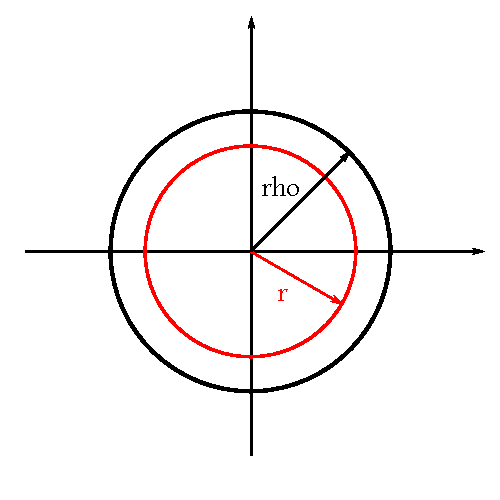
\includegraphics{img/convergence_radius.pdf}
    \caption{Convergence radius}
    \label{fig:convr}
  \end{center}
\end{figure}


\begin{rem}[An application of Theorem~\ref{thm:concl}]
  Let $P(z) = \sum_{k=0}^\infty a_k z^k$ be a power series with convergence radius $\rho(P)$ with
  \[ \rho(P) = \frac1L \qquad L = \limsup_{n\to\infty} \sqrt[n]{\abs{a_n}} \]
  \[ P_n(z) = \sum_{k=0}^n a_k z^k \qquad \text{\dots $n$-th partial sum} \]
  Let $r < \rho(P)$. Then it holds that $P_n(z) \to P(z)$ uniform in $\overline{B(0,r)}$~\footnote{Where overline means \enquote{closed}}.
  \[ P_n(x) \to P(x) \forall x \in [-r, r] \]

  Compare with Figure~\ref{fig:convr}.

  \[ P'_n(x) = \sum_{k=0}^n a_k k \cdot x^{k-1} = \sum_{j=0}^{n-1} a_{j+1} (j + 1) x^j \]
  is the $n-1$-th partial sum.
  \[ Q(z) = \sum_{j=0}^\infty a_{j+1} (j + 1) z^j \]
  Convergence radius of $Q$?
  \[ \tilde{L} = \limsup_{j\to\infty} \sqrt[j]{a_{j+1}} \cdot \sqrt[j]{j + 1} = \limsup_{j \to \infty} \abs{a_{j+1}}^{\frac{j+1}{j} \cdot \frac{1}{j+1}} \cdot (j+1)^{\frac{j+1}{j} \cdot \frac{1}{j+1}} \]
  \[
    = \limsup_{j\to\infty} \underbrace{\left(\abs{a_{j+1}}^{\overbrace{\frac{1}{j+1}}^{\to 1}}\right)^{\frac{j+1}{j}}}_{L^1 = L}
    \cdot \underbrace{\lim_{j\to\infty} \left[(j+1)^{\frac{1}{j+1}}\right]^{\frac{j+1}{j}}}_{1^1}
    = L
  \]
  In conclusion we have $\tilde L = L$ and $\rho(Q) = \frac1{L} = \rho(P)$.
  So $P'_n(z) = \sum_{k=1}^n k \cdot a_k z^{k-1}$ uniformly convergent in $\overline{B(0,r)}$ for $r<\rho$
  and therefore also uniformly convergent  in $[-r,r]$.

  From Theorem~\ref{thm:diff-conv} (or \ref{thm:concl}?) it follows that $P(x)$ is differentiable % TODO: or?
  in $[-r,r]$ and $P'(x) = \sum_{k=1}^\infty k \cdot a_k \cdot x^{k-1}$.

  Let $\abs{x} < \rho(P)$. Let $r = \frac12 (\abs{x} + \rho(P))$, then it holds that
  $x \in [-r, r]$ and $P$ is differentiable in point $x$ with
  \[ P'(x) = \sum_{k=1}^\infty k \cdot a_k \cdot x^{k-1} \]
\end{rem}

\begin{lemma}
  Let $P(z) = \sum_{k=0}^\infty a_k z^k$ be a power series with convergence radius $\rho(P) > 0$.
  Let $x \in (-\rho(P), \rho(P))$. Then $P$ is differentiable in $x$ and it holds that
  \[ P'(x) = \sum_{k=1}^\infty k \cdot a_k \cdot x^{k-1} \]

  Furthermore the power series $\sum_{k=1}^\infty k \cdot a_k \cdot x^{k-1}$ is uniformly convergent
  in every interval $[-r, r]$ with $0 < r < \rho(P)$.
\end{lemma}

\subsection{About logarithm functions}
%
We consider the power series
\[ g(z) = \sum_{k=1}^\infty \frac{z^k}{k} \]
\[ \rho(g) = \frac1L \text{ with } L = \limsup_{k\to\infty} \sqrt[k]{\frac1k} = \frac{1}{\lim_{k\to\infty} \sqrt[k]{k}} = 1 \]
So it holds that $\rho(g) = 1$.

Apply the previous theorem, followingly $g$ is differentiable in $(-1,1)$ and it holds that
\[ g'(x) = \sum_{k=1}^\infty \frac{k}{k} x^{k-1} = \sum_{j=0}^\infty x^j = \frac1{1 - x} \]

Remark:
\[ \left[-\ln(1 - x)\right]' = -\frac{1}{1 - x} \cdot (-1) = \frac1{1 - x} \]
\[ \Rightarrow \sum_{k=1}^\infty \frac{x^k}{k} + \ln(1 - x) = \text{ constant} \]
Let $x = 0$ (we determine the constant for this $x=0$):
\[ 0 + 0 = 0 = \text{ constant} \]
\[ \Rightarrow \ln(1 - x) = -\sum_{k=1}^\infty \frac{x^k}{k} \qquad \text{ for } \abs{x} < 1 \]

Let $x \in (-1,1) \Rightarrow -x \in (-1,1)$.
\[ \Rightarrow \ln(1 - (-x)) = \ln(1 + x) = -\sum_{k=1}^\infty \frac{(-x)^k}{k} \]
\[ = \sum_{k=1}^\infty \frac{(-1)^{k-1} \cdot x^k}{k} = x - \frac{x^2}{2} + \frac{x^3}{3} - \frac{x^4}{4} + \ldots \]

\index[English]{Logarithmic series}
\index[German]{\foreignlanguage{ngerman}{Logarithmische Reihe}}
Therefore: We introduce \emph{logarithmic series}:
\[ \ln(1 - x) = -\sum_{k=1}^\infty \frac{x^k}{k} \]
\[ \ln(1 + x) = \sum_{k=1}^\infty \frac{(-1)^{k-1} x^k}{k} \]
\[
  \ln\left(\frac{1 + x}{1 - x}\right)
  = \ln(1 + x) - \ln(1 - x)
  = 2 \sum_{l=1}^\infty \frac{x^{2l - 1}}{2l - 1}
  \quad \text{ for } x \in (-1,1)
\]

\begin{figure}[!h]
  \begin{center}
    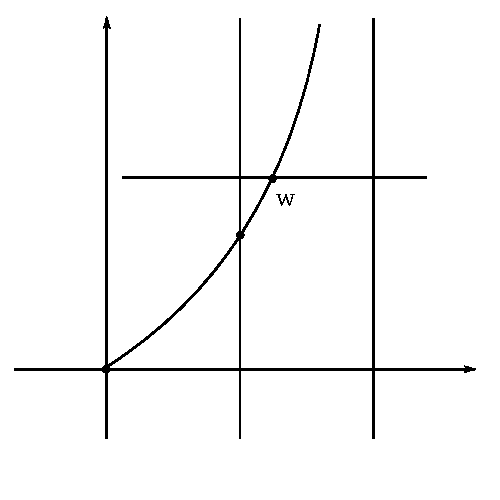
\includegraphics{img/1x_1-x.pdf}
    \caption{Plot of $\frac{1+x}{1-x}$}
    \label{img:1x-1x}
  \end{center}
\end{figure}

\[ f(x) = \frac{1 + x}{1 - x} \]
Compare with Figure~\ref{img:1x-1x}.
\[ f'(x) = \frac{1 - (-1)}{(1 - x)^2} = \frac{2}{(1 - x)^2} > 0 \quad \text{ in } (-1, 1) \]
Solve $\frac{1 + x}{1 - x} = w$ for $x$.

\[ \Rightarrow 1 + x  = w - wx \]
\[ x (1 + w) = w - 1 \]
\[ x = \frac{w - 1}{w + 1} \]

\[ \ln(w) = 2 \sum_{l=1}^\infty \frac{x^{2l-1}}{2l - 1} \]

\section{Trigonometic functions}

We define trigonometic functions using the exponential function in $\mathbb C$.

Let $t \in \mathbb R$.
\[ e^{it} = \sum_{k=0}^\infty \frac{(it)^k}{k!} = \lim_{n\to\infty} \left(\underbrace{1}_{\mathbb R} + \underbrace{\frac{it}{n}}_{i \mathbb R}\right)^n \]
\[
  e^{-it}
    = \lim_{n\to\infty} \left(1 - \frac{it}{n}\right)^n
    = \lim_{n\to\infty} \left[\overline{\left(1 + \frac{it}{n}\right)}\right]^n
\] \[
  = \lim_{n\to\infty} \overline{\left(1 + \frac{it}{n}\right)^n}
  = \overline{\lim_{n\to\infty} \left(1 + \frac{it}{n}\right)^n}
  = e^{it}
\] \[
  \abs{e^{it}}^2 = e^{it} \cdot \overline{e^{it}} = e^{it} \cdot e^{-it}
\] \[
  e^{it - it} = e^0 = 1
\]
So it holds that $\forall t \in \mathbb R$:
\[ \abs{e^{it}} = 1 \]
So $e^{it}$ lies inside the complex unit circle. Compare with Figure~\ref{img:unitc}.

\begin{figure}[!h]
  \begin{center}
    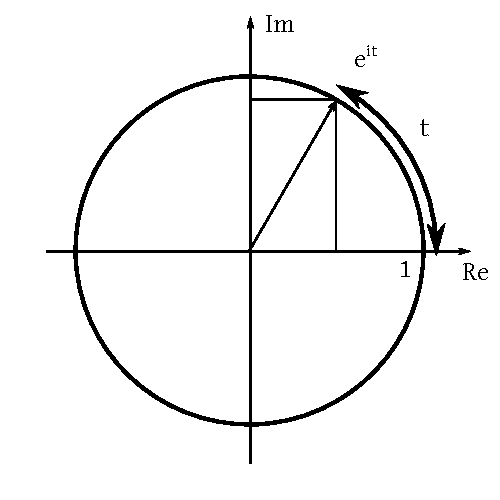
\includegraphics{img/unitcircle_in_C.pdf}
    \caption{Unit circle in $C$ with $t$}
    \label{img:unitc}
  \end{center}
\end{figure}

\index[English]{Sine function}
\index[German]{\foreignlanguage{ngerman}{Sinusfunktion}}
\index[English]{Cosine function}
\index[German]{\foreignlanguage{ngerman}{Cosinusfunktion}}
We define the cosine function $\cos: \mathbb R \to \mathbb R$ as
\[ \cos(t) = \Re(e^{it}) \]
and the sine function $\sin: \mathbb R \to \mathbb R$ as
\[ \sin(t) = \Im(e^{it}) \]

The following relations hold:
\begin{enumerate}
  \item $e^{it} = \cos(t) + i \cdot \sin(t)$ (Euler's identity)
  \item $\abs{e^{it}}^2 = 1 = (\cos{t})^2 + (\sin{t})^2$
  \item \[ \Re(z) = \frac12 (z + \overline{z}) \]
    \[ \Rightarrow \cos(t) = \Re(e^{it}) = \frac12 \left(e^{it} + e^{-it}\right) \]
    \[ \Im(z) = \frac1{2i} [z - \overline{z}] \]
    \[ \sin(t) = \Im(e^{it}) = \frac{1}{2i} \left[e^{it} - e^{-it}\right] \]
  \item
    \[ e^{-it} = \overline{e^{it}} = \cos{t} - i \cdot \sin{t} \]
\end{enumerate}

We use property 3 to extend the domain of sine and cosine:
\begin{defi}
  Let $z \in \mathbb C$. We define $\sin: \mathbb C \to \mathbb C$
  and $\cos: \mathbb C \to \mathbb C$ by
  \[ \cos(z) = \frac12 \left[e^{iz} + e^{-iz}\right] \]
  \[ \sin(z) = \frac1{2i} \left[e^{iz} - e^{-iz}\right] \]
\end{defi}

\meta{lecture}{8th of March 2016}{Wolfgang Ring}

\begin{figure}
  \begin{center}
    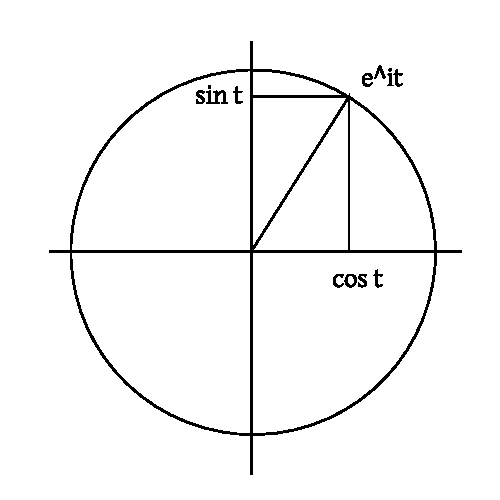
\includegraphics{img/complex_unit.pdf}
    \caption{The trigonometric values $\sin{t}$ and $\cos{t}$ in the unit circle}
    \label{img:cossin}
  \end{center}
\end{figure}
%
Compare with Figure~\ref{img:cossin}.

\begin{align*}
  t \in \mathbb R:
    \cos{t} = \Re(e^{it}) = \frac12 (e^{it} + e^{it}) \\
    \sin{t} = \Im(e^{it}) = \frac{1}{2i} (e^{it} - e^{-it})
\end{align*}

\begin{align*}
  z \in \mathbb C:
    \cos{z} &= \frac12 (e^{iz} + e^{-iz}) \\
    \sin{z} &= \frac{1}{2i} (e^{iz} - e^{-iz})
\end{align*}

Properties:
\begin{align*}
  \cos{-z} &= \frac12 (e^{i(-z)} + e^{-i}(-z)) = \cos{z} \\
  \intertext{$\cos{z}$ is even}
  \sin{-z} &= \frac1{2i} (e^{-iz} - e^{iz}) = -\sin{z}
  \intertext{$\sin{z}$ is odd}
\end{align*}

The cosine function in the complex space is even.

\subsection{Series representation of trigonometric functions}

\begin{lemma}[Addition of series of absolute convergence]
  Let $(a_n)_{n\in\mathbb N}$, $(b_n)_{n\in\mathbb N}$ be complex sequences
  and the series $\sum_{n=0}^\infty a_n$ and $\sum_{n=0}^\infty b_n$ are absolute
  convergent with series value $\sum_{n=0}^\infty a_n = a$ and $\sum_{n=0}^\infty b_n = s'$.

  Then $\sum_{n=0}^\infty (a_n + b_n)$ is absolute convergent with sum $s + s'$.
\end{lemma}
\begin{proof}[series sum]
  Absolute convergence.
  Show that $\sum_{k=0}^n = \abs{a_k + b_k} = t_n$ and $(t_n)_{n\in\mathbb N}$ is bounded.

  Follows immediately, because
  \[ \sum_{k=0}^n \abs{a_kk + b_k} \leq \underbrace{\sum_{k=0}^n \abs{a_k}}_{\text{bounded}} + \underbrace{\sum_{k=0}^n \abs{b_k}}_{\text{bounded}} \]
\end{proof}

\begin{ex}[Application]
  Let $P(z) \coloneqq \sum_{k=0}^\infty a_k z^k$ and $Q(z) \coloneqq \sum_{k=0}^\infty b_k z^k$ be power series.
  Both are convergent in $B(0, \delta)$. Then also $\sum_{k=0}^\infty (a_k + b_k) z^k$ is convergent in $B(0,\delta)$
  and it holds that $\sum_{k=0}^\infty (a_k + b_k) z^k = P(z) + Q(z)$.
\end{ex}

\subsection{Application to trigonometric functions}
%
\[ e^{iz} = \sum_{k=0}^\infty \frac{(iz)^k}{k!} = \sum_{k=0}^\infty i^k \cdot \frac{z^k}{k!} \]
\[ i^0 = 1 \qquad i^1 = i \qquad i^2 = -1 \qquad i^3 = -i \qquad i^4 = 1 = i^0 \qquad i^5 = i \qquad \ldots \]
\[ \Rightarrow = 1 + i \frac{z}{1!} - \frac{z^2}{2!} - i \frac{z^3}{3!} + \frac{z^4}{4!} + i \frac{z^5}{5!} - \frac{z^6}{6!} \]

\[ e^{-iz} = \sum_{k=0}^\infty \frac{(-iz)^k}{k!} = \sum_{k=0}^\infty (-i)^k \frac{z^k}{k!} \]
\[ (-i)^0 = 1 \qquad (-i)^1 = -i \qquad (-i)^2 = -1 \qquad (-i)^3 = i \qquad (-i^4) = 1 \qquad \ldots \]
\[ \Rightarrow = 1 - i \frac{z}{1!} - 1\frac{z^2}{2!} + i \frac{z^3}{3!} + \frac{z^4}{4!} - i \frac{z^5}{5!} - \frac{z^6}{6!} + \ldots \]

\[ \frac12 (e^{iz} + e^{-iz}) = 1 - \frac{z^2}{2!} + \frac{z^4}{4!} - \frac{z^6}{6!} + \frac{z^8}{8!} - \frac{z^{10}}{10!} + \ldots \]

Followingly,
\begin{align*}
  \cos{z} &= 1 - \frac{z^2}{2!} + \frac{z^4}{4!} - \frac{z^6}{6!} + \frac{z^8}{8!} - \ldots \\
          &= \sum_{l=0}^\infty (-1)^l \frac{z^{2l}}{(2l)!} \text{ convergent in } \mathbb C \\
  \sin{z} &= \frac1{2i}(e^{iz} - e^{-iz}) = z - \frac{z^3}{3!} + \frac{z^5}{5!} - \frac{z^7}{7!} + \frac{z^9}{9!} + \ldots \\
          &= \sum_{l=0}^\infty (-1)^l \frac{z^{2l + 1}}{(2l+1)!}
\end{align*}

\subsection{Functional equations of trigonometric functions}
%
\begin{theorem}[Addition and substraction theorems]
  We derive them directly:

  Let $z,w \in \mathbb C$.
  \begin{align*}
    e^{z+w} &= e^z \cdot e^w = (\cos{z} + i \cdot \sin{z}) (\cos{w} + i \cdot \sin{w}) \\
    \intertext{but also}
            &= (\cos(z + w) + i \sin(z + w)) \\
            &\Rightarrow = (\cos{z} \cdot \cos{w} - \sin{z} \cdot \sin{w}) + i (\cos{z} \cdot \sin{w} + \sin{z} c\dot \cos{w})
  \end{align*}

  Analogously,
  \begin{align*}
    e^{-(z+w)} &= e^{-z} \cdot e^{-w} = (\cos(-z) + i \cdot \sin(-z)) (\cos(-w) + i \cdot \sin(-w)) \\
               &= \cos{z} \cdot \cos{w} - \sin{z} \sin{w} + i \left(-\cos{z} \sin{w} - \cos{w} \sin{z}\right) \\
    \intertext{but also}
            &= (-\cos(z + w) + i \sin(-(z + w))) \\
            &\Rightarrow = \cos{(z + w)} - i \sin(z + w)
  \end{align*}

  \begin{align*}
    \intertext{Addition:} \\
    2 \cos(z+w) &= 2 (\cos{z} \cdot \cos{w} - \sin{z} \sin{w}) \\
    \Rightarrow \cos(z + w) &= \cos{z} \cos{w} - \sin{z} \sin{w}
    \intertext{Subtraction:}
    \Rightarrow \sin(z + w) &= \cos{z} \sin{w} + \sin{z} \cos{w} \forall z,w \in \mathbb C
  \end{align*}

  Variations: $w \leftrightarrow -w$
  \begin{align*}
    \cos(z - w) &= \cos{z} \cdot \underbrace{\cos{w}}_{=\cos(-w)} + \sin{z} \underbrace{\sin{w}}_{=-\sin(-w)} \\
    \sin(z - w) &= -\cos{z} \cdot \sin(w) + \sin(z) \cos(w)
  \end{align*}
\end{theorem}

\begin{cor}
  \[ z = \frac12 (z + w) + \frac12 (z - w) \]
  \[ \Rightarrow \cos{z} = \cos{\frac{z + w}{2}} \cos{\frac{z - w}{2}} - \sin{\frac{z + w}{2}} \sin{\frac{z - w}{2}} \]
  \[ w = \frac12 (w + z) + \frac12 (w - z) = \frac12 (z + w) - \frac12 (z - w) \]
  \[ \cos{w} = \cos{\frac{z + w}{2}} \cdot \cos{\frac{z - w}{2}} + \sin{\frac{z + w}{2}} \cdot \sin{\frac{z - w}{2}} \]
  \[ \cos{z} - \cos{w} = -2 \sin{\frac{z + w}{2}} \sin{\frac{z - w}{2}} \]
  Analogously,
  \[ \sin{z} - \sin{w} = 2 \cos{\frac{z + w}{2}} \cdot \cos{\frac{z - w}{2}} \]
\end{cor}

We consider
\begin{align*}
  \lim_{\substack{z \to 0 \\ z \neq 0}} \frac{\sin{z}}{z}
    &= \lim_{z \to 0} \frac{1}{2i} \left(\frac{e^{iz} - e^{-iz}}{z}\right) \\
    &= \lim_{z \to 0} e^{-iz} \left(\frac{e^{2iz} - 1}{2iz}\right) \\
    &= \underbrace{\lim_{z \to 0} e^{-iz}}_{=e^0 = 1} \cdot \underbrace{\lim_{z \to 0} \frac{e^{2iz} - 1}{2iz}}_{\substack{e = 2iz; z \to 0 \Leftrightarrow w = 0 \\ \lim_{w \to 0} \frac{e^w - 1}{w} = 1}}
\end{align*}

So it holds that
\[ \lim_{z\to0} \frac{\sin{z}}{z} = 1 \]

\subsection{Trigonometric functions for real arguments}
%
Subtitled \enquote{definition of $\pi$} and \enquote{periodicity}.

Let $x \in \mathbb R$.
\[ \cos{x} = \overbrace{1}^{=c_0} - \overbrace{\frac{x^2}{2}}^{=c_1} + \overbrace{\frac{x^4}{24}}^{=c_2} - \overbrace{\frac{x^6}{720}}^{=c_3} + \overbrace{\frac{x^8}{40320}}^{=c_4} - \ldots \]
\[ \sin{x} = \underbrace{x}_{=s_0} - \underbrace{\frac{x^3}{6}}_{=s_1} + \underbrace{\frac{x^5}{120}}_{=s_2} - \underbrace{\frac{x^7}{5040}}_{=s_3} + \ldots \]

\[ c_n = \frac{x^{2k}}{(2k)!} \qquad s_k = \frac{x^{2k+1}}{(2k+1)!} \]

For $x \in [0,2]$ and $k \geq 1$ it holds that
\[ \abs{\frac{c_{k+1}}{c_k}} = \abs{\frac{x^2}{(2k + 2)(2k + 1)}} \leq \frac{4}{3 \cdot 4} = \frac13 \]
so $(c_k)_{k\geq1}$ is strictly monotonically decreasing.

Leibniz criterion:
\[ 1 - \frac{x^2}{2} < \cos{x} < 1 - \frac{x^2}{2} + \frac{x^4}{24} \]
for $x \in (0,2]$.

Similarly for $x \in (0,2]$:
\[ \abs{\frac{s_{k+1}}{s_k}} = \abs{\frac{x^2}{(2k + 2)(2k + 3)}} \leq \frac{4}{4 \cdot 5} = \frac15 < 1 \]
So the Leibniz criterion tells us that
\[ x - \frac{x^3}{6} < \sin{x} < x \quad \text{ in } [0, 2] \]
So it holds that
\[ \cos(0) = 1 \]
\[ \cos(2) < 1 - 2 + \frac{16}{24} = -1 + \frac23 = -\frac13 \]
Intermediate value theorem (power series is continuous):
\[ \exists \xi \in (0,2) \text{ with } \cos(\xi) = 0 \]
Let $0 \leq w < z \leq 2$,
\[ 0 < \frac{z-w}{2} \leq \frac{z+w}{2} < \frac{z + z}{2} \leq 2 \]

Let $x \in (0,2]$, then it holds that
\[ \sin(x) > x - \frac{x^3}{6} = \underbrace{x}_{>0} \underbrace{\left(1 - \frac{x^2}{6}\right)}_{>1 - \frac46 = \frac13 > 0} > 0 \]
So it holds that $\sin(x) > 0$ in $(0,2]$.

Functional equation for $\cos{z} - \cos{w}$.
\[ \cos{z} - \cos{w} = \underbrace{-2  \cdot \underbrace{\sin{\underbrace{\frac{z+w}{2}}_{\in (0,2]}} \cdot \sin{\underbrace{\frac{z-w}{2}}_{\in (0,2]}}}_{>0}}_{<0} \]
$\cos{z} < \cos{w}$ for $0 \leq w < z \leq 2$.

So it holds that $\cos$ is a strictly monotonically decreasing functionin $[0,2)$. Hence $\cos$ has only one root because it is continuous in $(0,2]$.

\begin{defi}
  The number $\pi \in \mathbb R$ is defined as $\pi = 2\xi$, where $\xi$ is the uniquely defined root of the cosine in $(0,2]$.
\end{defi}

Some further important function values:
\[ 0 < \frac{\pi}{2} < 2 \text{ and } \cos{\frac\pi2} = 0 \]
because $\cos^2\left(\frac\pi2\right) + \sin^2\left(\frac\pi2\right) = 1$.
\[ \Rightarrow \abs{\sin\frac\pi2} = 1 \]
We know that $\sin{x} > 0$ for $x \in (0,2]$.
\[ \Rightarrow \sin\frac\pi2 = 1 \]

\[ e^{i \frac\pi2} = \cos\frac\pi2 + i \sin\frac\pi2 = i \]
\[ e^{i\pi} = e^{i\frac\pi2 + i\frac\pi2} = \left(e^{i\frac\pi2}\right)^2 = i^2 = -1 \]
\[ e^{i \frac32\pi} = e^{i\pi + \frac{i}2 \pi} = e^{i\pi} \cdot e^{i \frac\pi2} = -1 \cdot i = -i \]

Furthermore,
\[ e^{z + i\pi} = e^z \cdot \underbrace{e^{i\pi}}_{=-1} = -e^z \]
\[ e^{z + 2i\pi} = e^z \cdot \left(e^{i\pi}\right)^2 = e^z \]
So the exponential function is periodic in $\mathbb C$ with period $2i\pi$.

\begin{align*}
  \cos(z + 2\pi) &= \frac12 \left(e^{iz + 2\pi i} + e^{-iz - 2\pi i}\right) \\
    &= \frac12 \left(e^{iz} + e^{-iz} \cdot \underbrace{\frac1{e^{2\pi i}}}_{=1}\right) = \cos{z}
\end{align*}

Therefore the cosine is periodic in $\mathbb C$ with period $2\pi$.
Analogously, sine is periodic in $\mathbb C$ with period $2\pi$.

\meta{lecture}{10th of March 2016}{Wolfgang Ring}

\subsection{Periodicity and roots of trigonometric functions}

TODO: equations missing

\[ \cos(z + 2\pi) = \cos(z) \]
\[ \sin(z + 2\pi) = \sin(z) \]

\begin{table}
  \begin{tabular}{cccccc}
TODO: table missing &&&&&
  \end{tabular}
\end{table}

\begin{figure}[!h]
  \begin{center}
    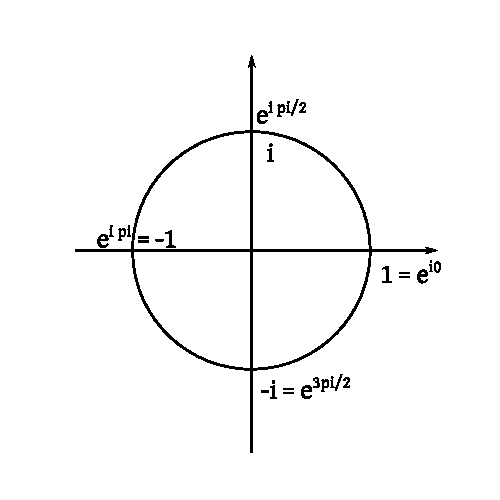
\includegraphics[width=0.5\textwidth]{img/trigonometric-periodicity.pdf}
  \end{center}
\end{figure}

\begin{rem}
  We will show: $\forall c \in (0, 2\pi)$, $\cos$ and $\sin$ are non-periodic with period $c$,
  hence $\exists x \in \mathbb R$ such that $\cos(x) \neq \cos(x + c)$.
\end{rem}

\index[English]{Periodic function}
\index[German]{\foreignlanguage{ngerman}{Periodische Funktion}}
\index[English]{Period}
\index[German]{\foreignlanguage{ngerman}{Periode}}
\begin{defi}
  \[ f: \mathbb C \to \mathbb C \qquad (f: \mathbb R \to \mathbb R) \]
  is called \emph{periodic} with period $c \in \mathbb C$ ($c \in \mathbb R$)
  if $\forall z \in \mathbb C$ it holds that
  \[ f(z + c) = f(z) \]
  \[ (\forall x \in \mathbb R: f(x + c) = f(x)) \]
  $c$ is called \emph{period of $f$}.
\end{defi}

\begin{rem}
  If $f$ is periodic with period $c \in \mathbb C$,
  then $f$ is also periodic with period $k \cdot c$ for every $k \in \mathbb Z \setminus \set{0}$.
\end{rem}

\begin{rem}
  \[ z = u + iv \]
  \[ \Re(i \cdot z) = \Re(i u - v) = -v = - \Im(z) \]
  \[ \Im(i \cdot z) = \Im(iu - v) = u = \Re(z) \]
\end{rem}

\begin{rem}
  Let $x \in \mathbb R$.
  \begin{align*}
    \cos\left(x + \frac\pi2\right)
      &= \Re(e^{i(x + \frac\pi2)}) \\
      &= \Re(e^{ix} \cdot e^{i\frac\pi2}) \\
      &= \Re(i e^{ix}) \\
      &= -\Im(e^{ix}) \\
      &= -\sin(x)
  \end{align*}

  \begin{align*}
    \sin\left(x + \frac\pi2\right)
      &= \Im\left(e^{i(x + \frac\pi2)}\right) \\
      &= \Im(ie^{ix}) \\
      &= \Re(e^{ix}) \\
      &= \cos(x)
  \end{align*}

  \begin{align*}
    \cos\left(x - \frac\pi2\right)
      &= \sin\left(x - \frac\pi2 + \frac\pi2\right) \\
      &= \sin(x)
  \end{align*}

  \begin{align*}
    \sin\left(x - \frac\pi2\right)
      &= -\cos\left(x - \frac\pi2 + \frac\pi2\right) \\
      &= -\cos(x)
  \end{align*}

  Summary:
  \begin{align*}
    \cos\left(x + \frac\pi2\right) &= -\sin(x) \\
    \sin\left(x + \frac\pi2\right) &= \cos(x) \\
    \cos\left(x - \frac\pi2\right) &= \sin(x) \\
    \sin\left(x - \frac\pi2\right) &= -\cos(x)
  \end{align*}
\end{rem}

\begin{rem}[A remark on the name \enquote{cosine}]
  \[ \sin\left(\frac\pi2 - x\right) = -\sin\left(x - \frac\pi2\right) = \cos(x) \]

  \begin{figure}[!h]
    \begin{center}
      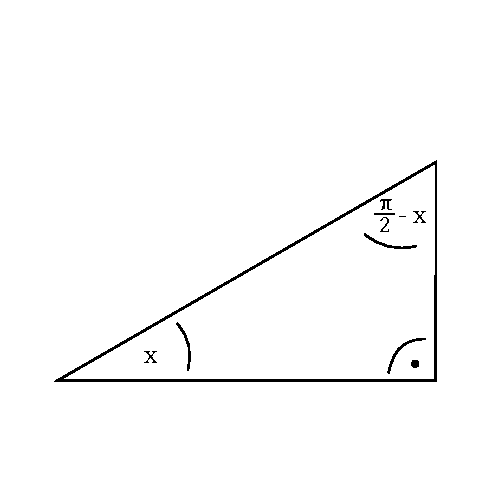
\includegraphics[width=0.4\textwidth]{img/complementary-angle.pdf}
      \caption{Complementary angle: co-sinus}
      \label{img:cosine}
    \end{center}
  \end{figure}

  The sine of the complementary angle is the co-sine of $x$ (Compare with Figure~\ref{img:cosine}).
\end{rem}

\begin{rem}
  \begin{align*}
    \cos(x + \pi) &= \Re(e^{i(x + \pi)}) \\
      &= \Re(-e^{ix}) \\
      &= -\cos(x) \\
    \sin(x + \pi) &= - \sin(x)
  \end{align*}
\end{rem}

\begin{rem}
  Let $0 < c < 2\pi$. Assume $\cos$ is periodic with period $c$.
  We know that $\cos$ has exactly one root in $[0,2]$,
  \[ \cos(x) = \cos(-x) \]
  $\cos$ has exactly two roots in $[-2,2]$, namely $\frac\pi2$ and $-\frac\pi2$.

  \begin{enumerate}
    \item Consider $c \in (0,\pi)$. Then $\cos\left(-\frac\pi2 + c\right) = \cos\left(-\frac\pi2\right) = 0$.
      \[ -\frac\pi2 + c < -\frac\pi2 + \pi = \frac\pi2 < 2 \]
      \[ -\frac\pi2 + c \geq -\frac\pi2 > -2 \]
      Therefore $\cos$ would have another root in $[-2,2]$, namely $-\frac\pi2 + c$.
      This is a contradiction.
    \item
      Consider $c \in [\pi,2\pi)$.
      $c = \pi$ is not a period because $\cos(0) = 1$ and $\cos(0 + \pi) = -1$.
      Let $\pi < c < 2\pi$.
      Then $\frac32 \pi - c < \frac32 \pi - \pi = \frac\pi2$ and $\frac32 \pi - c > \frac32 \pi - 2\pi = -\frac\pi2$.
      Hence,
      \[ \frac32 \pi - c \in \left(-\frac\pi2, \frac\pi2\right) \]
      \[ \cos\left(\frac32 \pi - c\right) = \cos\left(\frac32 \pi - c + c\right) = \cos\left(\frac32 \pi\right) = 0 \]
      $c$ would be the period.
      \[ \Rightarrow \frac32 \pi - c \text{ is a root of $\cos$ in } (-\frac\pi2, \frac\pi2) \]
      This is a contradiction.
  \end{enumerate}

  Therefore it holds that
  \[ \forall c \in (0,2\pi): \exists x \in \mathbb R: \cos(x + c) \neq \cos(x) \]
  Therefore $\cos$ is not periodic with period $c$.
  Hence $2\pi$ is indeed the smallest period of $\cos$.

  Analogously it holds for $\sin$.
\end{rem}

\begin{rem}[Roots of $\cos$]
  \[ \cos\left(\frac\pi2 + 2k\pi\right) = \cos\left(\frac\pi2\right) = 0 \qquad \forall k \in \mathbb Z \]
  \[ \cos\left(\frac32 \pi + 2k \pi\right) = \cos\left(\frac32 \pi\right) = 0 \qquad \forall k \in \mathbb Z \]
  \[ x_k = \frac\pi2 + 2k \pi = \frac{\pi}{2} \left(1 + 4k\right) \]
  \[ y_k = \frac32 \pi + 2k \pi = \frac\pi2 \left(3 + 4k\right) \]
  Hence for $z_l = \frac\pi2 \left(2l + 1\right)$ with $l \in \mathbb Z$ it holds that $\cos(z_l) = 0$.
  These are the odd multiples of $\frac\pi2$.

  \begin{align*}
    \sin(0 + 2k\pi) &= \sin(0) = 0 \\
    \sin(\pi + 2k\pi) &= \sin((2k + 1)\pi) = \sin(\pi) = 0
  \end{align*}
  \[ \Rightarrow (l\pi) = 0 \qquad \forall l \in \mathbb Z \]
\end{rem}

\subsection{Derivatives of trigonometric functions}
%
It holds that
\begin{mdframed}
  \[ \lim_{z \to 0} \frac{\sin{z}}{z} = 1 \]
\end{mdframed}
Furthermore it holds that
\begin{mdframed}
  \[ \lim_{z \to 0} \frac{1 - \cos{z}}{z} = 0 \]
\end{mdframed}

\begin{proof}
  \begin{align*}
    \frac{1 - \cos{z}}{z}
      &= \frac1z \left(1 - 1 + \frac{z^2}{2} - \frac{z^4}{4!} + \frac{z^6}{6!} - \frac{z^8}{8!} + \ldots\right) \\
      &= \frac{z}{2!} - \frac{z^3}{4!} + \frac{z^5}{6!} - \frac{z^7}{8!} + \ldots
  \end{align*}
  is convergent in $\mathbb C$ and (especially) continuous in $0$
  \[ \lim_{z \to 0} \left(\frac{z}{2!} - \frac{z^3}{4!} + \frac{z^5}{6!} - \ldots\right) = 0 \]
\end{proof}

\[
  \lim_{h\to0} \frac{\cos(x + h) - \cos(x)}{h}
\]

\meta{lecture}{11th of March 2016}{Wolfgang Ring}

Recall:
\[ \lim_{z\to0} \frac{\sin{z}}{z} = 1 \]
\[ \lim_{z\to0} \frac{1-\cos{z}}{z} = 0 \]

\begin{lemma}
  The trigonometric functions $\sin$ and $\cos$ are differentiable in $\mathbb R$
  (because they can be expressed as power series with infinite convergence radius)
  and it holds that
  \[ \cos'(x) = -\sin(x)  \qquad  \sin'(x) = \cos(x) \]
\end{lemma}
\begin{proof}
  \begin{align*}
    \lim_{h\to0} \frac{\cos(x + h) - \cos(h)}{h}
      &= \lim_{h\to0} \frac{\cos{x} \cdot \cos{h} - \sin{x} \cdot \sin{h} - \cos{x}}{h} \\
      &= \lim_{h\to0} \cos{x} \cdot \frac{\cos(h) - 1}{h} - \lim_{h\to0} \frac{\sin{x} \cdot \sin{h}}{h} \\
      &= \cos{x} \cdot \underbrace{\lim_{h\to0} \frac{\cos(h) - 1}{h}}_{=0} - \sin{x} \cdot \underbrace{\lim_{h\to0} \frac{\sin(h)}{h}}_{=1} \\
      &= -\sin(x)
  \end{align*}

  Analogously:
  \begin{align*}
    \lim_{h\to0} \frac{\sin(x + h) - \sin(h)}{h}
      &= \lim_{h\to0} \frac{\sin{x} \cdot \cos{h} + \sin{h} \cdot \cos{x} - \sin{x}}{h} \\
      &= \sin(x) \cdot \underbrace{\lim_{h\to0} \frac{\cos(h) - 1}{h}}_{=0} + \cos(x) \cdot \underbrace{\lim_{h\to0} \frac{\sin{h}}{n}}_{=1} \\
      &= \cos(x)
  \end{align*}
\end{proof}

TODO: incomplete graphics, verify text

\begin{figure}[!h]
  \begin{center}
    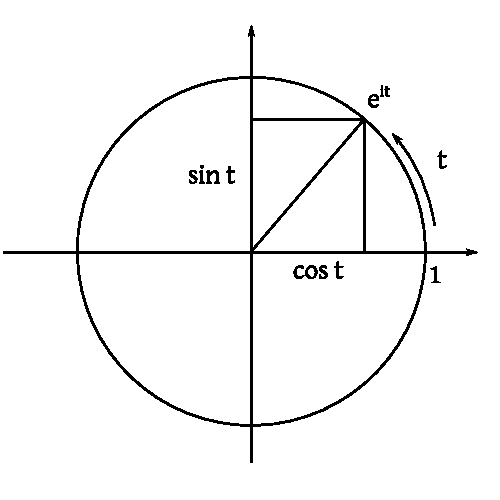
\includegraphics{img/arc-length-sincos.pdf}
    \caption{The arc length is related to $\sin$ and $\cos$}
    \label{img:arc-length}
  \end{center}
\end{figure}

Figure~\ref{img:arc-length}. We now use tools of integral calculus:

Let $I = [a,b]$ and $\gamma: I \to \mathbb R$ ($\mathbb R^2$).
\[ \gamma(t) = \begin{bmatrix} \gamma_1(t) \\ \vdots \\ \gamma_n(t) \end{bmatrix} \]
Assumption: $\gamma_1: [a,b] \to \mathbb R^n$.

\[ \gamma'(t) = \begin{bmatrix} \gamma'_1(t) \\ \vdots \\ \gamma'_n(t) \end{bmatrix} \]

TODO: graphics missing

Let $t \in [a,b]$. Then the arc length of $\gamma$ between $a$ and $t$
is given by
\[ S(t) = \int_a^t \abs{\gamma'(\tau)} \, d\tau \]

We identify $\mathbb C$ with $\mathbb R^2$:
\[ x + iy \leftrightarrow \begin{bmatrix} x \\ y \end{bmatrix} \]

\[ \gamma: t \mapsto e^{it} = \cos{t} + i \cdot \sin{t} \]
is a curve in $\mathbb C \cong \mathbb R^2$.
\[ \gamma: [0,2\pi] \to \mathbb C \]

\[ \gamma(t) = \begin{bmatrix} \cos{t} \\ \sin{t} \end{bmatrix} \]
\[ \gamma'(t) = \begin{bmatrix} -\sin{t} \\ \cos{t} \end{bmatrix} \]

\begin{figure}[!h]
  \begin{center}
    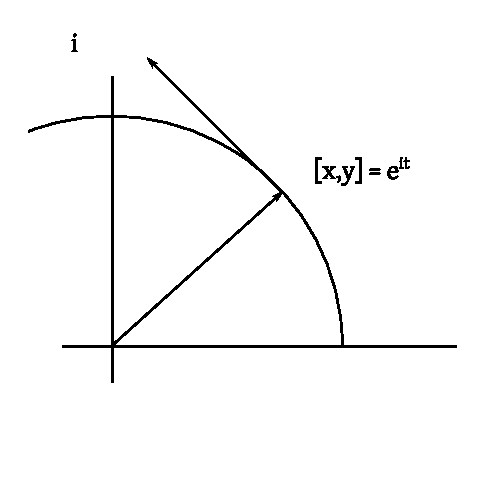
\includegraphics{img/derivative-in-r2.pdf}
    \caption{Derivative in $\mathbb R^2$}
    % TODO: incomplete
    \label{img:deriv-r2}
  \end{center}
\end{figure}

Compare with Figure~\ref{img:deriv-r2}.
\[ \abs{\gamma'(t)} = \sqrt{(-\sin(t))^2 + (\cos(t))^2} = 1 \]
\[ \int_0^t \abs{\gamma'(\tau)} \, d\tau = \int_0^t 1 \, d\tau = t \]

\section{Integration calculus}
%
Integration calculus was developed to determine areas of curves regions.
It was developed by Leibniz, Cauchy, Riemann and Lebeque. There are different
notions of integrations and it will discussed in further details in the courses
\enquote{Functional analysis} and \enquote{Measure and integration theory}.
For now, we look at the basis (as discussed by \foreignlanguage{ngerman}{Königsberger}).

\index[English]{Step function}
\index[German]{\foreignlanguage{ngerman}{Treppenfunktion}}
Let $[a,b]$ be an interval, $a,b \in \mathbb R$ with $a<b$ and $\phi: [a,b] \to \mathbb R$.
We call $\varphi$ a \emph{step function}, if $n \in \mathbb N$ and $x_0, \ldots, x_n$
exist such that
\[ x_0 = a < x_1 < x_2 < \ldots < x_n = b \]
and $\varphi|_{(x_{j-1}, x_j)} = c_j$ is constant.
The points $x_j$ define a partition of the interval $[a,b]$.

The function values defining the partitions do not have any constraints and
are therefore irrelevant for further considerations (compare with Figure~\ref{img:partition-int}).

\begin{figure}[!h]
  \begin{center}
    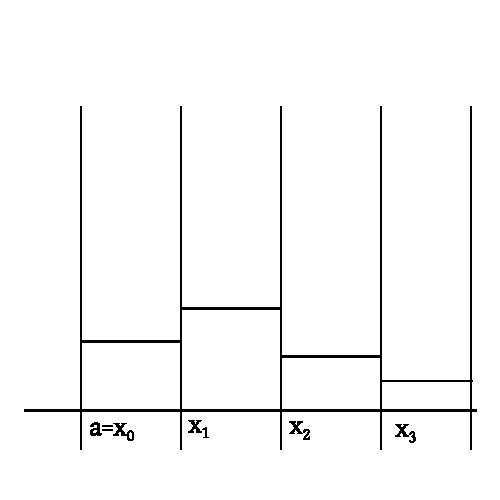
\includegraphics{img/partition-of-integral.pdf}
    \caption{Partition of an area into rectangles}
    \label{img:partition-int}
  \end{center}
\end{figure}

\index[English]{Integral}
\index[German]{\foreignlanguage{ngerman}{Integral}}
\begin{defi}
  Let $\varphi:[a,b] \to \mathbb R$ a step function and
  $x_0 = a < x_1 < \ldots < x_n = b$ as partition of
  $[a,b]$ and let $\varphi|_{(x_{j-1}, x_j)} = c_j$
  for $j = 1,\ldots,n$.
  Then we define
  \[ \int_a^b \varphi \,dx = \sum_{j=1}^n c_j \triangle x_j \]
  where
  $\triangle x_j = x_j - x_{j-1}$ (for $j=1,\ldots,n$).
  \[ \int_a^b \varphi \, dx \text{ is called \emph{integral} of $\varphi$ over $[a,b]$} \]
\end{defi}

$\varphi$ is the step function in terms of the partition $\set{x_0,x_1,\ldots, x_5}$.

It remains to show that if $\varphi$ satisfies the definition of a step function in terms of
partition $\set{x_0,\ldots,x_n}$ and $\varphi|_{(x_{j-1}, x_j)} = c_j$
(TODO: text missing: \enquote{but \ldots})
and $\varphi$ is a step function in terms of $\set{w_0,w_1,\ldots,w_m}$
and $\varphi|_{(w_{l-1},w_l)} = c'_l$, then it holds that
\[ \sum_{j=1}^n c_j \triangle x_j = \sum_{l=1}^m c'_l \triangle w_l \]
Compare with Figure~\ref{img:step-function}.

\begin{figure}[!h]
  \begin{center}
    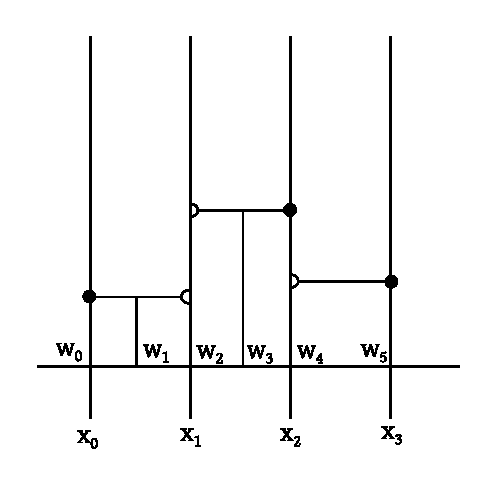
\includegraphics{img/step-function.pdf}
    \caption{Step function $\varphi$}
    \label{img:step-function}
  \end{center}
\end{figure}

% TODO: verify
\begin{proof}
  Let $Z = \set{x_0, \ldots, x_n}$ and $Z' = \set{w_0,\ldots,w_m}$.
  We define $Z'' = Z \cup Z'$ and $Z'' = \set{\alpha_0, \alpha_1, \ldots, \alpha_L}$.
  Duplicates get lost in the set.
  \[ \alpha_0 = a < \alpha_1 < \ldots < \alpha_L = b \]
  Because $Z \subseteq Z''$,
  \[ \forall x_j \exists k_j: x_j = \alpha_{k_j} \]
  Because $x_{j-1} < x_j$, it holds that $\alpha_{k_{j-1}} < \alpha_{k_j}$.
  Followingly,
  \[ k_{j-1} < k_j \]
  Let $k_{j-1} < l \leq k_j$.
  It holds that $(\alpha_{l-1}, \alpha_l) \subseteq (x_{j-1}, x_j)$,
  because $l > k_{j-1} = l-1 \geq k_{j-1} \Rightarrow \alpha_{l-1} \geq \alpha_{k_{j-1}} = x_{j-1}$
  and $l \leq k_j$.
  \[ \Rightarrow \alpha_l \leq \alpha_{k_j} = x_j \]
  So for $x \in (\alpha_{l-1}, \alpha_l) \subseteq (x_{j-1}, x_j)$ it holds that
  $\varphi(x) = c_j$.

  $k_0 = 0$ because $x_0 = \alpha_0 = a$ and $k_n = L$ because $x_n = \alpha_L = b$.
  $\forall l \in \set{0,\ldots,L}$ there exists $j \in \set{1,\ldots,n}$ such that
  $k_{j-1} \leq l \leq k_j$.

  \[ \Rightarrow \varphi|_{(\alpha_{l-1},\alpha_l)} \text{ is constant} \]

  Hence $\varphi$ is a step function in terms of the partition $\set{\alpha_0, \ldots, \alpha_L}$.

  Let $l \in \set{0,1,\ldots,L}$ and $j$ such that
  \[ k_{j-1} < l \leq k_j \Rightarrow (\alpha_{l-1},\alpha_l) \subset (x_{j-1},x_j) \]
  and $c''_l = \varphi(x)$ for $x \in (\alpha_{l-1},\alpha_l)$, then $c''_l = c_j$.

  \[ \sum_{l=1}^L c''_l \cdot \triangle \alpha_l = \sum_{j=1}^n \sum_{l=k_{j-1}+1}^{k_j} c''_l \triangle \alpha_l \]
  \[ = \sum_{j=1}^n c_j \sum_{l=k_{j-1}}^{k_j} \triangle \alpha_l \]
  \[ \sum_{l=k_{j-1} + 1}^{k_j} \triangle \alpha_l = (\alpha_{k_{j-1}+1} - \alpha_{k_{j-1}})
    + (\alpha_{k_{j-1}+2} - \alpha_{k_{j-1}+1}) + (\alpha_{k_{j-1}+3} - \alpha_{k_{j-1}+2})
  \] \[
    + \ldots + (\alpha_{k_j-1} - \alpha_{k_j-2}) + (\alpha_{k_j} - \alpha_{k_j-1})
  \]
  This is a telescoping sum. What remains is:
  \[ = \alpha_{k_j} - \alpha_{k_{j-1}} \]

  \[ x_j - x_{j-1} = \triangle x_j \]
  Analogously,
  \[ \sum_{l=1}^L c''_l \cdot \triangle \alpha_l = \sum_{k=1}^m c'_k \triangle w_k \]
  So it holds that
  \[ \sum_{j=1}^n c_j \triangle x_j = \sum_{k=1}^m c'_k \triangle w_k \]
\end{proof}

\clearpage
\begin{otherlanguage}{ngerman}
\printindex[German]
\end{otherlanguage}
\printindex[English]

\end{document}

%%% Local Variables:
%%% mode: latex
%%% TeX-master: t
%%% End:
